\documentclass[12pt,a4paper]{article}




\usepackage{float}
\usepackage{polyglossia}
\usepackage{graphicx,wrapfig,lipsum}
\usepackage{xspace}
\usepackage{glossaries}
\usepackage{color}
\usepackage{fontspec}

\usepackage{blindtext}
\usepackage[utf8]{inputenc}
\usepackage{fancyhdr}

\usepackage{booktabs} %for Excel
\usepackage{multirow}
\usepackage{pbox}

\usepackage{hyperref}

\usepackage{siunitx}
\usepackage{comment}
\usepackage{enumitem}
\usepackage{amsmath}

\usepackage{tabularx} % for table adjustment
%
\usepackage[a4paper ,total={6in, 8in}]{geometry}
%\usepackage[showframe=true]{geometry}
% XeLaTeX!
% ============================================================ %
% HEBREW support via polyglossia %
% ============================================================ %
%\usepackage{polyglossia}
\defaultfontfeatures{Mapping=tex-text, Scale=MatchLowercase}
\setdefaultlanguage{english}
\setotherlanguage{hebrew}
\newfontfamily\hebrewfont[Script=Hebrew]{David}
% Use \begin{hebrew} block of text \end{hebrew} for paragraphs.
% Use \texthebrew{ } and \textenglish{ } for short texts.
% ============================================================ %
\newcommand{\te}[1]{\textenglish{#1}}


\newcommand{\thh}[1]{\texthebrew{#1}}
%Hyper Link Setup
\hypersetup{
	colorlinks=true,
	linkcolor=blue,
	filecolor=magenta,      
	urlcolor=blue,
}

%% DMM and link to wiki
\newcommand{\dmm}{\href{https://en.wikipedia.org/wiki/Multimeter}{\te{(DMM)}}}

\begin{document}
	\begin{hebrew}
		\title{ספק כוח}
		\maketitle
	\end{hebrew}
\pagebreak
	\begin{hebrew}
		\section{רקע כללי}
		ספק כוח הוא יחידה אלקטורנית שתפקידה לספק למעגלים אלקטרוניים את המתח והזרם החשמלי הדרושים להפעלתם. \\
		במעגל זרם ישר, יכול ספק הכוח לשמש כמקור מתח או מקור זרם, לפי הצורך. בדרך כלל מאופיין ספק הכוח על ידי מתח מסוים וכן זרם מרבי אותו הוא מסוגל לספק ללא ירידה במתח, או לחלופין את ההספק שהוא מסוגל לתת. ההזנה לספקי כוח יכולה להיות למשל מרשת החשמל הביתית, מצבר או סוללות.
		\section{סוגי מכשירי מעבדה}
		\begin{enumerate}
			\item
			\te{GPS - 3303}
			\begin{figure}[h] 
				\centering
				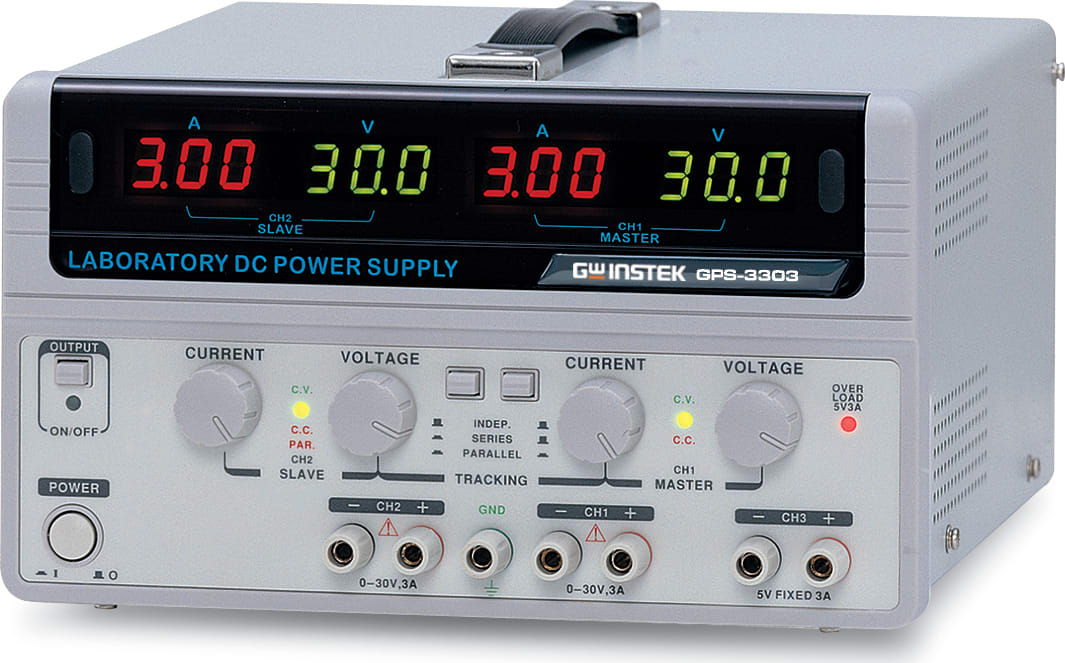
\includegraphics[width=0.7\linewidth]{../Figure/GPS-3303}
			%	\caption{}
			%	\label{fig:gps-3303}
			\end{figure}	
		\end{enumerate}
\pagebreak
	\begin{hebrew}
		\section{פירוט על כל דגם}
		\subsection{GPS-3303}

\begin{figure}[h]
	\centering
	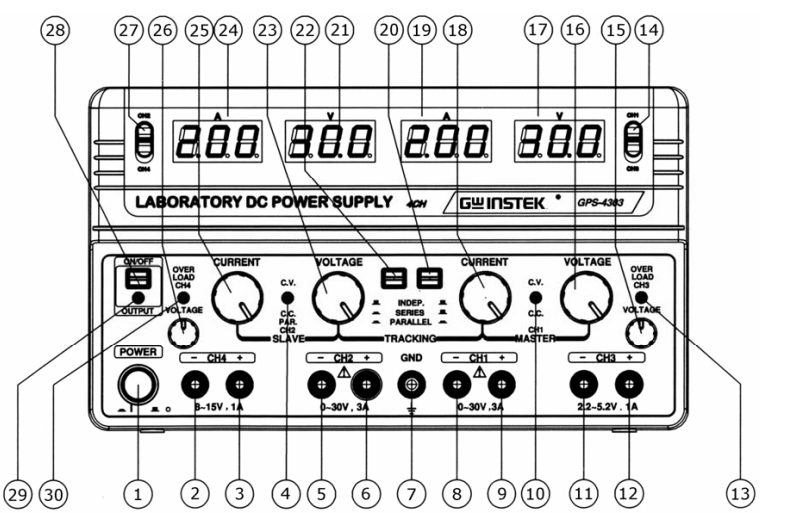
\includegraphics[width=0.7\linewidth]{../Figure/description}
%	\caption{}
	\label{fig:description}
\end{figure}

\begin{enumerate}
	\item
	כפתור הפעלה.
	\addtocounter{enumi}{2}
	\item
	\te{CH2,SLAVE}
	מנורת סימון : \\
	ירוק  = מתח קבוע.\\
	אדום = זרם קבוע.
	\item
	\te{CH2,SLAVE}
	- מחבר יציאה.
	\item
	\te{CH2,SLAVE}
	 + מחבר יציאה.
	 \item
	 \te{GND}
	 מחבר יציאת אדמה.
	 \item
	 \te{CH1,MASTER}
	 - מחבר יציאה.
	 \item
	 \te{CH1,MASTER}
	 + מחבר יציאה.
	 \item
	\te{CH1,MASTER}
מנורת סימון : \\
ירוק  = מתח קבוע.\\
אדום = זרם קבוע.	
	\item
	\te{CH3,CONST:$ \SI{5}{\volt} , \SI{3}{\ampere} $}
	- מחבר יציאה.
		\item
	\te{CH3,CONST:$ \SI{5}{\volt} , \SI{3}{\ampere} $}
	+ מחבר יציאה.
	\item
	\te{CH3,CONST:$ \SI{5}{\volt} , \SI{3}{\ampere} $}
	מנורת סימון שדולק.
	\addtocounter{enumi}{2}
	\item
	
	בורר של \te{CH1,MASTER} מתח.
	\item
	צג מתח,זרם של \te{CH1,MASTER}
	\item
	בורר של \te{CH1,MASTER} זרם.
	\addtocounter{enumi}{1}
	\item
	.22 שליטה של שלושה מצבים :\\
	מצב עצמי(שני הכפתורים משוחררים). \\
	מצב טורי(רק כפתור שמאלי לחץ). \\
	מצב מקבילי(שני הכפתורים לחוצים). 
	
	\item 
	צג מתח,זרם \te{CH2,SLAVE}.
	\addtocounter{enumi}{1}
	\item
		בורר של \te{CH2,SLAVE} מתח.
	\addtocounter{enumi}{1}
	\item
		בורר של \te{CH2,SLAVE} זרם.
	
	\begin{hebrew}
	 	לפירוט נוסף אפשר לפנות ל:
	 	\href{https://www.manualslib.com/manual/811590/Gw-Instek-Gps-2303.html?page=9#manual}{\te{User Manual}}
	\end{hebrew}
	 
	 
\end{enumerate}
	\end{hebrew}
		
	\end{hebrew}
\end{document}